\documentclass{classrep}
\usepackage[utf8]{inputenc}
\frenchspacing

\usepackage{graphicx}
\usepackage[usenames,dvipsnames]{color}
\usepackage[hidelinks]{hyperref}
\usepackage{lmodern}
\usepackage{graphicx}
\usepackage{placeins}
\usepackage{url}
\usepackage{amsmath, amssymb, mathtools}
\usepackage{listings}
\usepackage{fancyhdr, lastpage}

\pagestyle{fancyplain}
\fancyhf{}
\renewcommand{\headrulewidth}{0pt}
\cfoot{\thepage\ / \pageref*{LastPage}}

%--------------------------------------------------------------------------------------%
\studycycle{Informatyka stosowana, studia dzienne, II st.}
\coursesemester{II}

\coursename{Przetwarzanie i analiza dużych zbiorów danych}
\courseyear{2021/2022}

\courseteacher{mgr inż. Rafał Woźniak}
\coursegroup{Czwartek, 15:45}

\author{%
    \studentinfo[239661@edu.p.lodz.pl]{Szymon Gruda}{239661}\\
    \studentinfo[239671@edu.p.lodz.pl]{Jan Karwowski}{239671}\\
    \studentinfo[239673@edu.p.lodz.pl]{Michał Kidawa}{239673}\\
    \studentinfo[239676@edu.p.lodz.pl]{Kamil Kowalewski}{239676}\\
}

\title{Checkpoint 1}

\begin{document}
    \maketitle
    \thispagestyle{fancyplain}

    \tableofcontents
    \newpage

    \section{Wprowadzenie} {
        Głównym celem projektu jest przeprowadzenie kompleksowej analizy zbioru
        \textit{NYPD Complaint Data Historic} \cite{nypd_dataset}. Jego dokładny opis
        został umieszczony w sekcji \ref{dataset_description} natomiast jego cele oraz
        pytania na które będziemy chcieli znaleźć odpowiedź w trakcie wykonywania
        analizy zostały przedstawione w sekcji \ref{project_goals}.
    }

    \section{Podział obowiązków w zespole} {
        \begin{itemize}
            \item Szymon Gruda - Przygotowanie statystycznego opisu zbioru danych dla
            danych określonych jako lokalizacja zdarzenia, cechy podejrzanego i
            ofiary oraz zależności między podejrzanym a ofiarą. Dodatkowo udział
            w grupowych rozważaniach.
            \item Jan Karwowski - sformułowanie w przystępny sposób opisu celów
            przygotowanych przez zespół. Dodatkowo udział w grupowych rozważaniach.
            \item Michał Kidawa - Przygotowanie opisu kolumn oraz zebranie w formie
            tekstowej informacji o wstępnym przetwarzaniu danych. Dodatkowo
            udział w grupowych rozważaniach.
            \item Kamil Kowalewski - Przygotowanie ogólnego opisu danych zbioru oraz
            statystycznego opisu zbioru danych dla danych określonych jako data i
            czas zgłoszenia, typ i opis wykroczenia, status przestępstwa (czy się
            udało) oraz otoczenie zdarzenia. Dodatkowo udział w grupowych
            rozważaniach.
        \end{itemize}
    }

    \section{Statystyczny opis zbioru danych} \label{dataset_description} {
        \subsection{Opis kolumn} {
            Zbiór danych zawiera kolumny których nazwy oraz opisy w pogrupowany sposób
            zostały przedstawione poniżej:
        % @formatter:off
            \begin{enumerate}
                \item Identyfikator
                \begin{itemize}
                    \item CMPLNT\_NUM - Losowo generowany trwały identyfikator dla każdego zgłoszenia
                \end{itemize}
                \item Data i czas zdarzenia
                \begin{itemize}
                    \item CMPLNT\_FR\_DT - Dokładna data wystąpienia zgłoszonego zdarzenia (lub data początkowa wystąpienia, jeżeli CMPLNT\_TO\_DT istnieje)
                    \item CMPLNT\_FR\_TM - Dokładny czas wystąpienia zgłoszonego zdarzenia (lub czas rozpoczęcia wystąpienia, jeżeli CMPLNT\_TO\_TM istnieje)
                    \item CMPLNT\_TO\_DT - Data końcowa wystąpienia zgłoszonego zdarzenia, jeżeli dokładny czas wystąpienia nie jest znany
                    \item CMPLNT\_TO\_TM - Końcowy czas wystąpienia zgłoszonego zdarzenia, jeżeli dokładny czas wystąpienia nie jest znany
                \end{itemize}
                \item Data i czas zgłoszenia
                \begin{itemize}
                    \item RPT\_DT - Data zgłoszenia zdarzenia na policję
                \end{itemize}
                \item Typ i opis wykroczenia/przestępstwa
                \begin{itemize}
                    \item KY\_CD - Trzycyfrowy kod klasyfikacji wykroczeń
                    \item OFNS\_DESC - Opis wykroczenia odpowiadający kodowi klucza
                    \item PD\_CD - Trzycyfrowy kod klasyfikacji wewnętrznej (bardziej szczegółowy niż Key Code)
                    \item PD\_DESC - Opis wewnętrznej klasyfikacji odpowiadającej kodowi PD (bardziej szczegółowy niż opis przestępstwa)
                    \item LAW\_CAT\_CD - Poziom wykroczenia: przestępstwo, wykroczenie, naruszenie
                \end{itemize}
                \item Czy się udało
                \begin{itemize}
                    \item CRM\_ATPT\_CPTD\_CD - Status, czy przestępstwo zostało dokonane czy była próba jego popełnienia lub czy zostało ono przerwane
                \end{itemize}
                \item Otoczenie zdarzenia
                \begin{itemize}
                    \item PREM\_TYP\_DESC - Rodzaj otoczenia; sklep spożywczy, domek jednorodzinny, ulica itp.
                    \item LOC\_OF\_OCCUR\_DESC - Lokalizacja w stosunku do otoczenia; wewnątrz, naprzeciw, z przodu, z tyłu
                \end{itemize}
                \item Lokalizacja zdarzenia
                \begin{itemize}
                    \item ADDR\_PCT\_CD - Posterunek
                    \item BORO\_NM - Dzielnica
                    \item JURIS\_DESC - Opis kodu jurysdykcji
                    \item JURISDICTION\_CODE - Kod jurysdykcji na której miało miejsce to zdarzenie
                    \item PARKS\_NM - Nazwa parku, placu zabaw lub terenów zielonych w Nowym Jorku, jeśli dotyczy (parki stanowe nie są uwzględnione)
                    \item HADEVELOPT - Nazwa osiedla NYCHA miejsca zdarzenia, jeśli dotyczy
                    \item HOUSING\_PSA - Kod poziomu rozwoju
                    \item X\_COORD\_CD - Współrzędna X dla układu współrzędnych płaszczyzny stanu Nowy Jork, strefa Long Island, NAD 83, jednostki w stopach (FIPS 3104)
                    \item Y\_COORD\_CD - Współrzędna Y dla układu współrzędnych płaszczyzny stanu Nowy Jork, strefa Long Island, NAD 83, jednostki w stopach (FIPS 3104)
                    \item TRANSIT\_DISTRICT - Okręg tranzytowy, w którym doszło do wykroczenia.
                    \item Latitude - Współrzędna szerokości geograficznej środkowego bloku dla globalnego układu współrzędnych, WGS 1984, stopnie dziesiętne (EPSG 4326)
                    \item Longitude - Współrzędna długości bloku środkowego dla globalnego układu współrzędnych, WGS 1984, stopnie dziesiętne (EPSG 4326)
                    \item Lat\_Lon - Punkt lokalizacji geoprzestrzennej (łącznie szerokość i długość geograficzna)
                    \item PATROL\_BORO - Nazwa dzielnicy patrolowej, w której doszło do incydentu
                    \item STATION\_NAME - Nazwa stacji tranzytowej
                \end{itemize}
                \item Cechy podejrzanego
                \begin{itemize}
                    \item SUSP\_AGE\_GROUP - Grupa wiekowa podejrzanego
                    \item SUSP\_RACE - Rasa podejrzanego
                    \item SUSP\_SEX - Płeć podejrzanego
                \end{itemize}
                \item Cechy ofiary
                \begin{itemize}
                    \item VIC\_AGE\_GROUP - Grupa wiekowa ofiary
                    \item VIC\_RACE - Rasa ofiary
                    \item VIC\_SEX - Płeć ofiary
                \end{itemize}
            \end{enumerate}
        % @formatter:on
        }
        
        \subsection{Wykresy} {

            \subsubsection{Data i czas zgłoszenia} {

                \begin{figure}[!htbp]
                    \centering
                    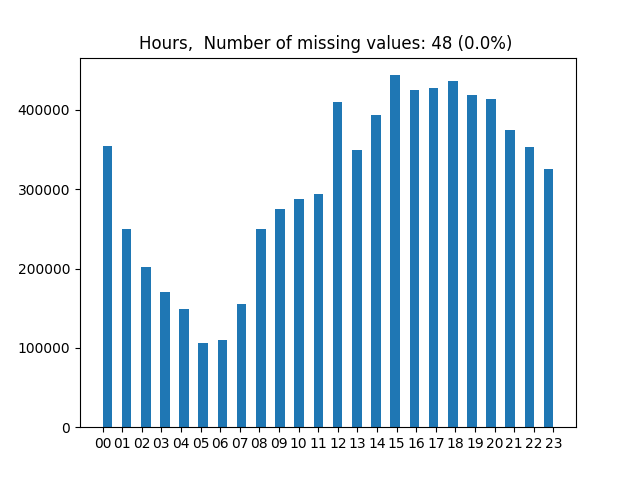
\includegraphics[width=\textwidth]{img/Hours-133549.png}
                    \caption{Histogram liczby przestępstw w zależności od godziny}
                    \label{hist_hours}
                \end{figure}
                \begin{figure}[!htbp]
                    \centering
                    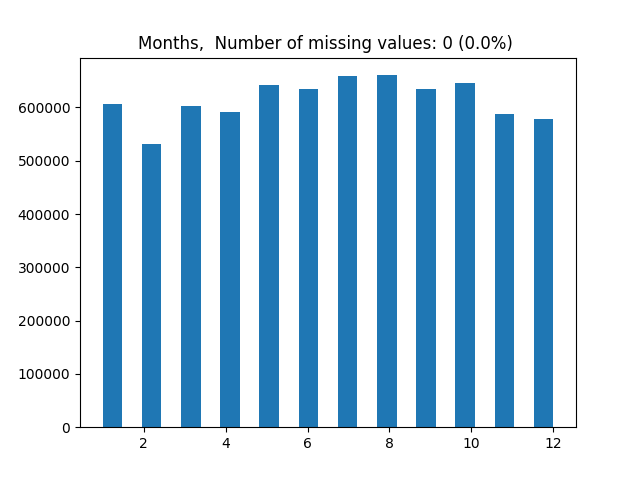
\includegraphics[width=\textwidth]{img/Months-133554.png}
                    \caption{Histogram liczby przestępstw w zależności od miesiąca}
                    \label{hist_months}
                \end{figure}
                \FloatBarrier

                Na podstawie rysunku \ref{hist_hours} można zaobserwować, że największa
                liczba przestępstw/wykroczeń miała miejsce w godzinach popołudniowych,
                natomiast najmniejsza w godzinach wczesnoporonnych tzn godzina 5 i 6 rano.

                Na podstawie rysunku \ref{hist_months} można zaobserwować, że wyniki
                liczby przestępstw/wykroczeń są do siebie zbliżone natomiast większa
                liczba była w czasie miesięcy letnich.

                Dla rekordów w, których występuję wartość \emph{CMPLNT\_TO\_DT} oraz
                \emph{CMPLNT\_TO\_TM} została obliczony średni czas między początkiem a
                końcem zdarzenia i są to następujące wartości
                \begin{itemize}
                    \item średnia: 8 days 21:03:19.644759679
                    \item odchylenie standardowe: 190 days 21:44:14.282341806
                \end{itemize}

                Dla rekordów została policzony średni czas oraz odchylenie standardowe
                w dniach między wystąpieniem zdarzenia a jego zgłoszeniem na policje i
                są to następujące wartości:
                \begin{itemize}
                    \item średnia: 14 days 19:01:46.072720350
                    \item odchylenie standardowe: 233 days 01:34:24.475636108
                \end{itemize}
            
            }

            \subsubsection{Typ i opis wykroczenia/przestępstwa} {
                \begin{figure}[!htbp]
                    \centering
                    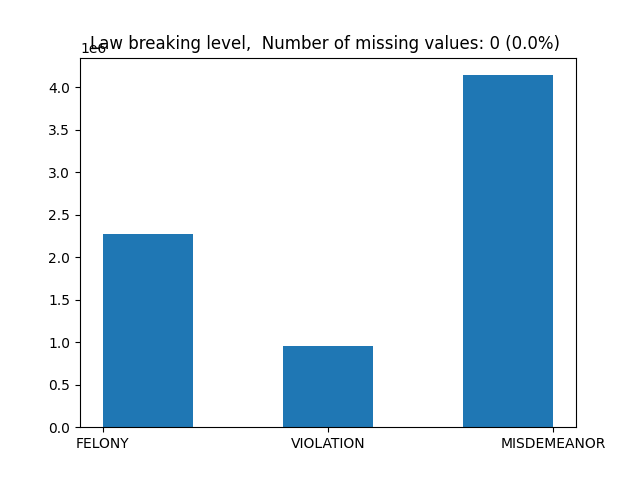
\includegraphics[width=0.9\textwidth]{img/Lawbreakinglevel-133608.png}
                    \caption{Histogram liczby przestępstw/wykroczeń zależnie od jego typu}
                    \label{hist_law_breaking_level}
                \end{figure}
                \FloatBarrier

                Na podstawie rysunku \ref{hist_law_breaking_level} można zaobserwować,
                że największy odsetek stanowiły wykroczenia, na drugim miejscu
                uplasowały się przestępstwa natomiast najmniej było występków(jest to
                pośredni czy miedzy wykroczeniem a przestępstwem).
            }

            \subsubsection{Czy się udało} {
                \begin{figure}[!htbp]
                    \centering
                    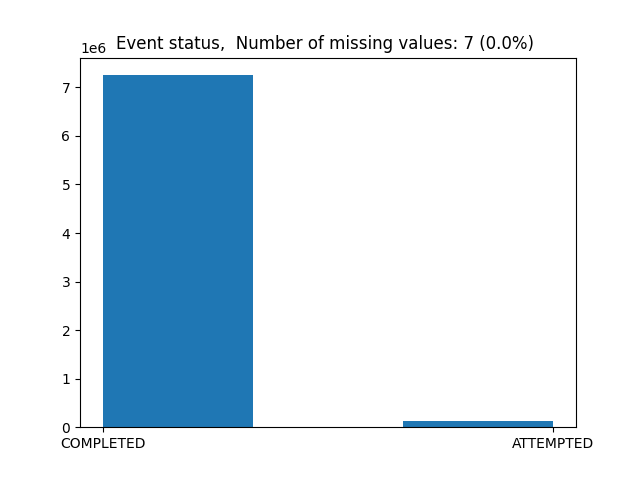
\includegraphics[width=0.75\textwidth]{img/Eventstatus-133630.png}
                    \caption{Histogram liczby przestępstw/wykroczeń w zależności od tego czy doszło ono do skutku czy zostało zatrzymane}
                    \label{hist_is_completed}
                \end{figure}
                \FloatBarrier
                Na podstawie rysunku \ref{hist_is_completed} można zaobserwować, że
                praktycznie wszystkie przestępstwa/wykroczenia zostały dokonane a
                naprawdę niewielki odsetek został udaremniony.
            }

            \subsubsection{Otoczenie zdarzenia} {
                \begin{figure}[!htbp]
                    \centering
                    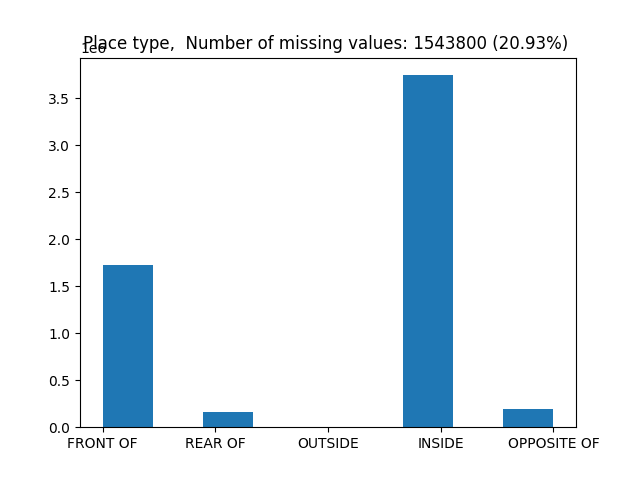
\includegraphics[width=\textwidth]{img/Placetype-133640.png}
                    \caption{Histogram liczby przestępstw/wykroczeń w zależności od typu miejsca w jakim się zdarzyło}
                    \label{hist_place_type}
                \end{figure}
                \FloatBarrier
                Na podstawie rysunku \ref{hist_place_type} można zaobserwować, że wg
                raportów policji znakomita większość miała miejsce w środku danego
                miejsca, drugim najczęściej wskazanym otoczeniem było miejsce przed np.
                danym budynkiem.
            }

            \subsubsection{Lokalizacja zdarzenia} {
                \begin{figure}[!htbp]
                    \centering
                   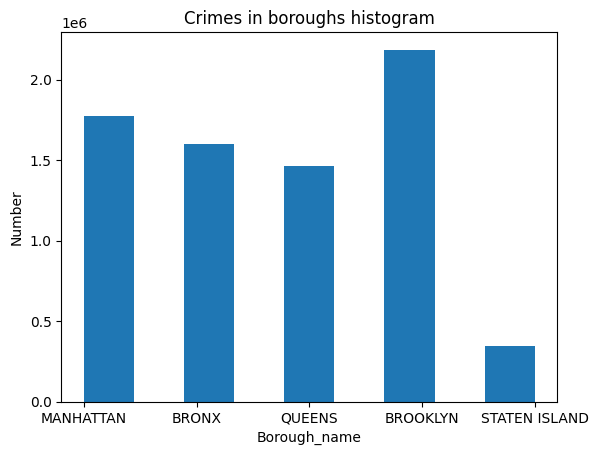
\includegraphics[width=\textwidth]{img/3.2.5/Borough_name#Number-084440.png}
                    \caption{Histogram liczby przestępstw w zależności od dzielnicy}
                    \label{borough_hist}
                \end{figure}
                \FloatBarrier
                Na podstawie rysunku \ref{borough_hist}. można zobaczyć, że w dzielnicy
                Brooklyn dochodzi do największej liczby przestępstw, w Staten Island
                najmniej, natomiast pozostałe dzielnice posiadają podobną liczbę
                popełnionych przestępstw. Przyczyną odbiegających od nich wyników dla
                Brooklyn'u i Staten Island może być, np. ich powierzchnia.
            }

            \subsubsection{Cechy podejrzanego} {
                \begin{figure}[!htbp]
                    \centering
                    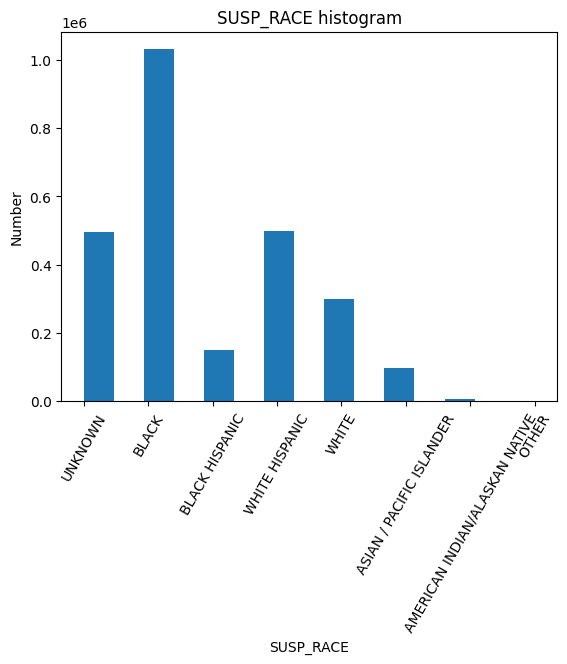
\includegraphics[width=\textwidth]{img/3.2.6/SUSP_RACE#Number-084449.png}
                    \caption{Histogram liczby przestępstw popełnianych przez określoną rasę.}
                    \label{susp_race}
                \end{figure}
                \begin{figure}[!htbp]
                    \centering
                    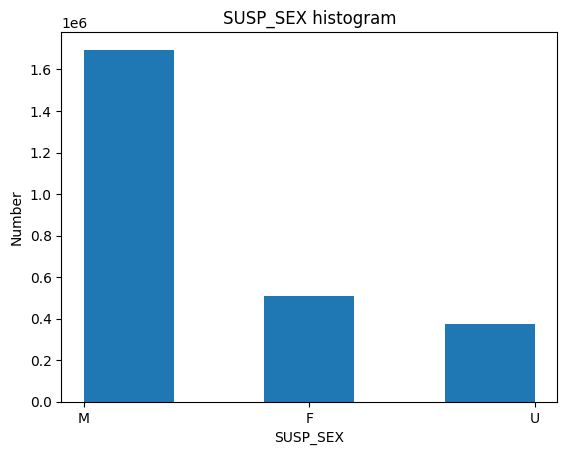
\includegraphics[width=\textwidth]{img/3.2.6/SUSP_SEX#Number-084454.png}
                    \caption{Histogram liczby przestępstw popełnianych przez określoną płeć.}
                    \label{susp_sex}
                \end{figure}
                \FloatBarrier
                Na podstawie rysunków \ref{susp_race}. i \ref{susp_sex} można zauważyć,
                że najwięcej podejrzanych o przestępstwo cechuje się czarnym kolorem
                skóry, lub płcią męską. Dysproporcje pomiędzy rasą, mogą być
                spowodowane np. nierównym procentowym udziałem tych ras w społeczeństwie.
            }

            \subsubsection{Cechy ofiary} {
                 \begin{figure}[!htbp]
                    \centering
                    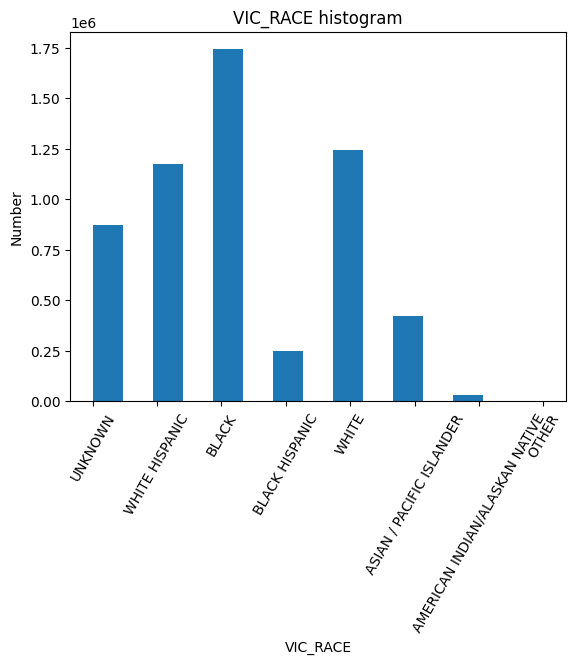
\includegraphics[width=\textwidth]{img/3.2.7/VIC_RACE#Number-084509.png}
                    \caption{Histogram liczby przestępstw, których ofiarą jest określona rasa.}
                    \label{vic_race}
                \end{figure}
                \begin{figure}[!htbp]
                    \centering
                    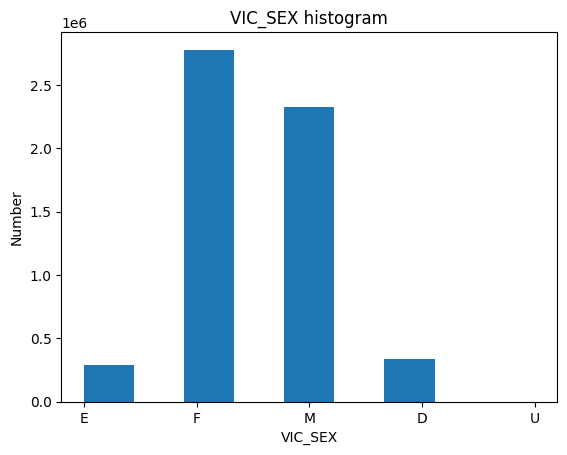
\includegraphics[width=\textwidth]{img/3.2.7/VIC_SEX#Number-084517.png}
                    \caption{Histogram liczby przestępstw, których ofiarą jest określona płeć.}
                    \label{vic_sex}
                \end{figure}
                \FloatBarrier

                Na podstawie rysunków \ref{vic_race}. i \ref{vic_sex} można zauważyć,
                że najwięcej ofiar przestępstw cechuje się czarnym kolorem skóry, lub
                płcią żeńską (chociaż nie ma dużej różnicy pomiędzy nią, a płcią męską)
                . Dysproporcje pomiędzy rasą, mogą być spowodowane np. nierównym
                procentowym udziałem tych ras w społeczeństwie. Albo cechami
                społeczności, niektóre osoby z pewnego powodu, mogą nie czuć obowiązku
                zgłaszania przestępstwa.
            }
            
            \subsubsection{Zależności między podejrzanym a ofiarą} {
                \begin{figure}[!htbp]
                    \centering
                    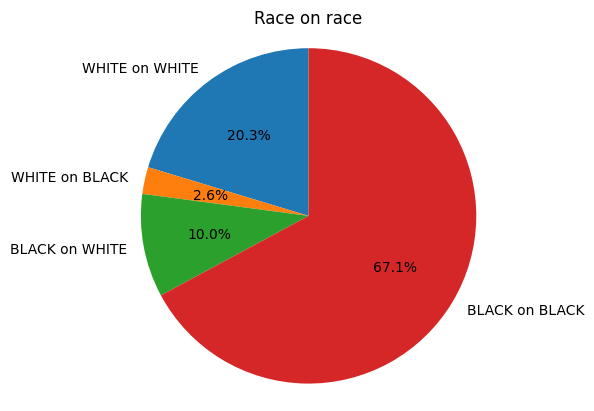
\includegraphics[width=\textwidth]{img/3.2.8/Race#piechart-084518.png}
                    \caption{Wykres przedstawiający zależność pomiędzy podejrzanym a ofiarą, na podstawie ich rasy (uwzględnione zostały tylko dwie).}
                    \label{pie_chart_race}
                \end{figure}
                \begin{figure}[!htbp]
                    \centering
                    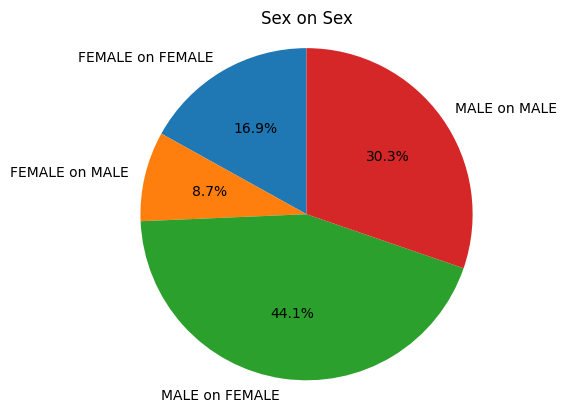
\includegraphics[width=\textwidth]{img/3.2.8/Sex#piechart-084518.png}
                    \caption{Wykres przedstawiający zależność pomiędzy podejrzanym a ofiarą, na podstawie ich płci (uwzględnione zostały tylko dwie).}
                    \label{pie_chart_sex}
                \end{figure}
                \FloatBarrier

                Do wykresów \ref{pie_chart_race} i \ref{pie_chart_sex} zostały wybrane
                dwie rasy i płcie, które największą liczbę razy uczestniczyły w
                przestępstwie jako ofiara lub podejrzany. W ten sposób się
                zaobserwować, że największy odsetek przestępstw dotyczył tej samej
                rasy, można zatem stwierdzić, że odsetek przestępstw między rasowych
                jest niższy niż można było się spodziewać. Natomiast sprawdzenie
                rozkładu płci, nie zaskutkowało niespodziewanymi wnioskami. Mężczyźni
                ogólnie częściej są podejrzanymi o przestępstwa i częściej popełniają
                takie, w których ofiarami są kobiety niż mężczyźni.
            }
        }


    }

    \section{Cele projektu} \label{project_goals} {
        W ramach projektu sformułowane zostały trzy następujące cele.

        \subsection{Klasyfikacja rodzaju lub poziomu przestępstwa}
        \label{project_goal_1} {

            W ramach tego etapu przeprowadzony zostanie szereg eksperymentów mających
            na celu stworzenie klasyfikatora typu przestępstwa (KY\_CD). Jeżeli okaże
            się to niemożliwe podjęta zostanie próba klasyfikacji poziomu wykroczenia,
            stanowiącego bardziej ogólną informacje. Klasyfikacja ta będzie odbywała
            się na podstawie następujących informacji:
            \begin{itemize}
                \item godzina zdarzenia
                \item dzień tygodnia zdarzenia
                \item odstęp między zgłoszeniem a zdarzeniem
                \item czy doszło do skutku (CRM\_ATPT\_CPTD\_CD)
                \item otoczenie zdarzenia
                \item cechy podejrzanego
                \item cechy ofiary
                \item poziom lub typ przestępstwa w zależności od tego co klasyfikujemy
            \end{itemize}

            Wybrane cechy mogą ulec drobnym modyfikacjom w trakcie trwania
            eksperymentów. Opcjonalnie podjęta będzie próba wykorzystania informacji o
            czasie trwania przestępstwa (dla tych zdarzeń, dla których jest dostępna).

            Informacja o dokładnej lokalizacji zdarzenia nie jest wykorzystana ze
            względu na chęć stworzenia uniwersalnego narzędzia.

            Aby zrealizować zaproponowany cel wykorzystane zostaną następujące metody:
            metody imputacji brakujących danych, prosta ekstrakcja cech (zwłaszcza z
            daty), naiwny klasyfikator Bayesa i lasy losowe.
        }

        \subsection{Klasyfikacja wieloetykietowa cech podejrzanego}
        \label{project_goal_2} {

            Kolejnym celem będzie klasyfikacja cech podejrzanego (wieku, rasy, płci) na
            podstawie:
            \begin{itemize}
                \item godzina zdarzenia
                \item dzień tygodnia zdarzenia
                \item odstęp między zgłoszeniem a zdarzeniem
                \item czy doszło do skutku (CRM\_ATPT\_CPTD\_CD)
                \item typ i waga przestępstwa
                \item otoczenie zdarzenia
                \item cechy ofiary
            \end{itemize}
            W przeciwieństwie do poprzedniego celu, tym razem klasyfikacja będzie miała
            charakter wieloetykietowy, to znaczy klasyfikator będzie przypisywał
            zdarzeniu kilka klas jednocześnie. Wykorzystane zostaną dedykowane
            klasyfikatory, pozwalające przypisywać wiele klas do pojedynczego
            przykładu, jak ML-KNN czy sieć neuronowa. Alternatywnie mogą zostać użyte
            klasyfikatory dające jedną etykietę, jak klasyczny las losowy, a samo
            zadanie klasyfikacji wieloetykietowej zostanie podzielone na wiele podzadań
            klasyfikacji binarnych.
        }

        \subsection{Grupowanie przestępstw na podstawie podzbiorów cech}
        \label{project_goal_3} {
            W ramach tego celu przeprowadzone zostanie automatyczne grupowanie zdarzeń.
            Spośród cech podejrzanego i ofiary kilkakrotnie wybrany zostanie podzbiorów
            stanowiących przedmiot eksperymentu - etykietę. Dla każdej wybranej
            etykiety (która może być złożeniem kilku atrybutów) przeprowadzona zostanie
            seria eksperymentów, mająca na celu automatyczne pogrupowanie zdarzeń
            zgodnie z tą etykietą, wykorzystując wszystkie pozostałe atrybuty (poza
            tworzącymi etykietę). Po przeprowadzeniu grupowania z wykorzystaniem kilku
            różnych algorytmów (DBSCAN, k-means, algorytm aglomeracyjny), zmierzona
            zostanie jakość grupowania za pomocą metryk zewnętrznych (accuracy)
            względem wybranej etykiety. Dodatkowo porównana zostanie jakość grupowania
            między seriami eksperymentów (dla różnych etykiet) za pomocą metryk
            wewnętrznych.
        }

    }

    \section{Wstępne przetwarzanie danych} {
        Do wstępnego przetwarzania danych został wykorzystany język Python oraz
        biblioteka Pandas. Za ich pomocą zostało wygenerowane podsumowanie zbioru
        poprzez wywołanie funkcji \emph{describe()}, pomogła ona w znalezieniu
        zależności oraz wybraniu ciekawych danych do prezentacji na wykresach i
        histogramach. W przypadku przegotowywania danych do histogramów gdy występowała
        pusta wartość była ona pomijana.
    }

    \begin{thebibliography}{0}
        % @formatter:off
        \bibitem{nypd_dataset}{https://data.cityofnewyork.us/Public-Safety/NYPD-Complaint-Data-Historic/qgea-i56i}
        % @formatter:on
    \end{thebibliography}

\end{document}
